\documentclass[xcolor=table]{beamer}

\usepackage{shyne}

% Theme settings
\setbeamertemplate{navigation symbols}{}

\usetheme{Madrid}
\usefonttheme{structurebold}
\usefonttheme[onlymath]{serif}

\AtBeginSection[]
{ 	\begin{frame}{}

	{
	\usebeamerfont{frametitle}
	\begin{beamercolorbox}
		[wd={\textwidth}, center, sep=.2in, rounded=true, shadow=true]
		{frametitle}
	Chapter \thesection\\  \secname 
	\end{beamercolorbox}
	}
	
	\end{frame} 
}

\AtBeginSubsection[]
{ 	\begin{frame}{}

	{
	\usebeamerfont{frametitle}
	\begin{beamercolorbox}
		[wd={\textwidth}, center, sep=.2in, rounded=true, shadow=true]
		{frametitle}
	Section \thesection .\thesubsection\\  \subsecname 
	\end{beamercolorbox}
	}
	
	\end{frame} 
}

\title[Chapter 7]{Stat 201: Statistics I\\ Chapter 7 }
\author[M. Shyne]{}
\institute[Metro State]{
\includegraphics[width=1.75in]{../images/metro_logo}}
\date[Feb 26, 2018]{Februaury 26, 2018
\\ \bigskip \bigskip 
\includegraphics[width=.4in]{../images/cc_big}}


\begin{document}
\frame{\titlepage}

% Chapter 7
\setcounter{section}{6}
\section{Estimating Parameters and Determining Samples Sizes}

\begin{frame}{Confidence intervals}
\begin{block}{}
\large Recall, sample statistics can be used as estimators for population parameters. However, estimators are rarely exactly equal to the parameter.\\
\pause\medskip
 It is more informative to calculate a \bt{confidence interval}, a range of values that is likely to contain the value of the parameter.
\end{block}

\end{frame}

\begin{frame}{Components of confidence intervals}
\begin{block}{}
\large
A confidence interval, defined for a specific confidence level, is constructed with a point estimate and a margin of error.
\end{block}
\pause
\begin{block}{}
\large A \bt{confidence level} is an indication of the level of certainty that the interval will contain the true parameter. 
\end{block}
\pause
\begin{block}{}
\large The \bt{point estimate} is the value the estimator, the sample statistic used to estimate the population parameter. For example, $\bar x$.
\end{block}
\pause
\begin{block}{}
\large The \bt{margin of error} is the amount the lower and upper bounds of the interval differ from the point estimate.
\end{block}
\end{frame}

\begin{frame}{Confidence levels}

\begin{block}{}
\large
The confidence level is the probability that a confidence interval constructed from a random sample actually contains the true population parameter.\\
\begin{itemize}
\pause\item Expressed as a percent, in terms of $\alpha$ as $(1-\alpha)\%$
\pause\item It would be incorrect to say: ``There is a 95\% chance the true parameter is in the interval."
\pause\item Rather: ``We are 95\% confident that the interval contains the true parameter."
\item Or: ``When constructing intervals from random samples with this method, 95\% of the time the interval will contain the true parameter."
\end{itemize} 
\end{block}

\end{frame}

\begin{frame}{Margin of error}
\begin{block}{}
\large
The margin of error can be thought of as the amount of uncertainty in an estimate. It is calculated in the context of the sampling distribution, the confidence level and the sample standard deviation and size.
\pause\[ME = z_{\alpha/2} \Paren{\frac s {\sqrt n}}\]
Where...
\begin{itemize}
\item $z_{\alpha/2}$ is the two sided critical $z$ value at $\alpha$ level of significance  
\item $s$ is the sample standard deviation
\item $n$ is the sample size
\end{itemize}
\end{block}
\end{frame}

\begin{frame}{Critical values}
\begin{block}{}
\large
Recall, for a significance level $\alpha$, the critical values $z_{\alpha/2}$ and $-z_{\alpha/2}$ separate the bulk of the distribution from the lowest and highest values comprising a total proportion of $\alpha$ of the distribution.\\
\medskip
Thus, between the critical values is an area or probability of $(1-\alpha)$. 
\end{block}
\medskip
{\centering
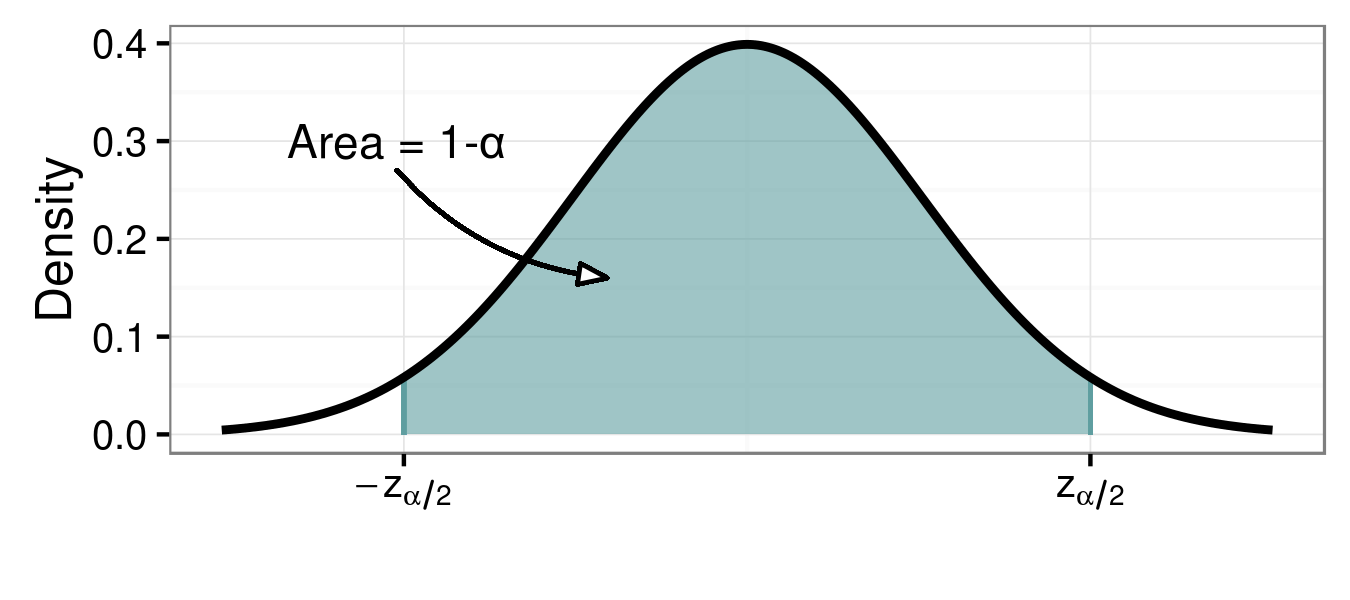
\includegraphics[width=4.5in]{../images/ch7_crit_values}
\par}
\end{frame}

\begin{frame}{Standard normal critical values}
\begin{block}{}
\large
{\centering
\begin{tabular}{c | c | c }
Sig. Level ($\alpha$) & Conf. Level ($1-\alpha$)  & Critical Value ($z_{\alpha/2}$)\\
\hline
0.10 & 90\% &  1.645\\
0.05 & 95\% & 1.96 \\
0.01 & 99\% & 2.576
\end{tabular}
\par}
\end{block}
\end{frame}

\begin{frame}{Confidence interval definition}

\begin{block}{}
\large
A confidence interval at confidence level $(1-\alpha)$\%, given a sample of size $n$ with point estimate $x$ and standard deviation $s$, is
\[CI (1-\alpha)\% = x \pm ME = x \pm z_{\alpha/2}\Paren{\frac s {\sqrt n}}\]
or
\[\Paren{x - z_{\alpha/2}\Paren{\frac s {\sqrt n}}, x + z_{\alpha/2}\Paren{\frac s {\sqrt n}} }\]
\end{block}

\end{frame}

\begin{frame}{Inference using confidence intervals}
\begin{block}{}
\large
If a confidence interval does not contain a value of interest, then it can be said there is evidence that the sample was drawn from a population whose parameter is different than the value of interest.
\end{block}

\pause
\begin{exampleblock}{Example}
Recall, in the United States, adult men have a mean height of 69.2 in with a standard deviation of 5.79 in. \\
\medskip
If a confidence interval for mean height calculated from a sample of male Metro State students is $(62.3, 67.9)$, then there is evidence that male Metro State students are shorter then the general US population.
\end{exampleblock}
\end{frame}

\begin{frame}{Find point estimate and margin of error}
\begin{block}{}
\large
Given a confidence interval $(L_{ci}, U_{ci})$, the point estimate and margin of error can be calculated.
\[\text{Point estimate: } x = \frac {L_{ci} + U_{ci}}{2}\]
\[\text{Margin of error: } ME = \frac {U_{ci} - L_{ci}}{2}\]
\end{block}

\medskip
{\centering
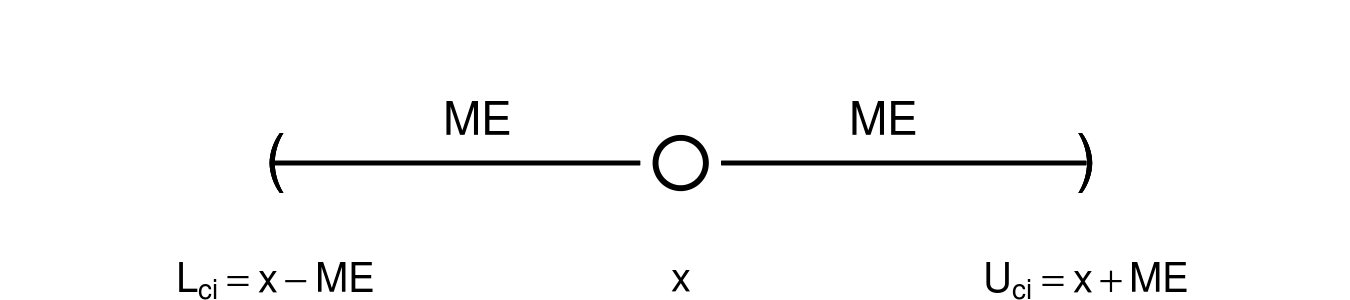
\includegraphics[width=4.5in]{../images/ch7_ci_numline}
\par}

\end{frame}

\begin{frame}{Find point estimate and margin of error, example}
\begin{exampleblock}{Example}
From the previous example, we had a confidence interval for the heights of male Metro State students of $(62.3, 67.9)$ or $62.3 < \mu < 67.9$.\\
\medskip
 What is the point estimate and margin of error of this confidence interval?\\
\medskip
\begin{itemize}
\pause\item Point estimate:\\
\smallskip
{\centering
$\ds \bar x = \frac {L_{ci} + U_{ci}}{2} = \frac {62.3 + 67.9}{2} = 65.1$ inches
\par}
\smallskip
\pause\item Margin of error:\\
\smallskip
{\centering
$\ds ME = \frac {U_{ci} - L_{ci}}{2} = \frac {67.9 - 62.3}{2} = 2.8$ inches
\par}
\smallskip
\pause\item So we can state this confidence interval as\\
\smallskip
{\centering
$\ds \bar x \pm ME \implies 65.1 \pm 2.8$ inches
\par}

\end{itemize}
\medskip
\end{exampleblock}

\end{frame}

\begin{frame}{Sample size}
\begin{block}{}
\large
When designing experiments, sample sizes are determined in order to achieve a desired accuracy. In other words, an acceptable margin of error is used to calculate the needed sample size.\\
\pause\medskip
Using the previous definition of margin of error,
\[ME = z_{\alpha/2} \Paren{\frac s {\sqrt n}}\]
after some algebra,
\[ n = \Paren{\frac {s \times z_{\alpha/2}}{ME}}^2\]
\end{block}
\end{frame}

% Section 7.1
\subsection{Estimating a Population Proportion}

\begin{frame}{Population proportions}
\begin{block}{}
\large
Recall, a population proportion $p$ can be estimated by the point estimate of the sample proportion $\hat p$ which follows a normal distribution.
\begin{itemize}
\pause\item More precisely, a sample proportion follows a binomial distribution, which approximates a normal distribution as $n$ increases.
\pause\item The variance of $\hat p$ is $s^2 = \hat p (1-\hat p) = \hat p \hat q$
\pause\item The standard deviation of $\hat p$ is $s = \sqrt{\hat p \hat q}$
\end{itemize}
\end{block}
\end{frame}

\begin{frame}{Confidence intervals of proportions}
\begin{block}{}
\large
A confidence interval of a population proportion with confidence level $(1-\alpha)$\% from a sample of size $n$ and sample proportion $\hat p$ is
\[CI = \hat p \pm ME = \hat p \pm z_{\alpha/2} \sqrt{\frac {\hat p \hat q}{n}}\]
\end{block}
\end{frame}

\begin{frame}{Confidence intervals of proportions in StatCrunch}
\begin{block}{}
\begin{itemize}
\item Stat $\to$ Proportion Stats $\to$ One Sample $\to$ With Summary
\item Enter ``\# of successes" and ``\# of observations"
\item Select ``Confidence interval for p"
\item Enter confidence level if different than 0.95.
\item Click ``Compute!"
\item The confidence interval is found in ``L. Limit" and ``U. Limit"
\end{itemize}
\end{block}
\end{frame}


\begin{frame}{Confidence intervals of proportions, example}
\begin{exampleblock}{Example}
\large
Suppose 100 Metro State students were asked if they had eaten a taco in the past week. 36 students responded they had in fact eaten a taco. What is a 95\% confidence interval for the proportion of all Metro State students who have eaten a taco in the past week.
\begin{itemize}
\pause\item 95\% confidence level means $\alpha = 0.05$
\pause\item $\ds \hat p = \frac {36}{100} = 0.36$
\pause\item $\ds ME = z_{\alpha/2}\sqrt{\frac {\hat p \hat q}{n}} = (1.96)\sqrt{\frac {(0.36)(0.64)}{100}} = 0.094$
\pause\item $\ds CI = \hat p \pm ME = 0.36 \pm 0.094 = (0.266, 0.454)$
\end{itemize}
\pause We are 95\% confident that the true proportion of Metro State students who have eaten a taco in the last week in between 0.266 and 0.454.
\end{exampleblock}
\end{frame}


\begin{frame}{Inference of population proportion}
\begin{block}{}
\large
A confidence interval can be used to make inferences about a population that a sample is drawn from by testing whether the CI contains a known value.\\
\pause\medskip
For example,
\begin{itemize}
\item To test whether a sub-population is similar to the larger population
\item To test whether an intervention changed attitudes, actions or outcomes
\end{itemize}

\pause If the known parameter value (the proportion of the larger population, or the proportion before the intervention) \bt{is not} contained in the confidence interval, it can be said there is evidence of a change.\\
\medskip
If the known value \bt{is} within the interval, then there is not evidence of a difference.
\end{block}
\end{frame}

\begin{frame}{Inference of population proportion, example}
\begin{exampleblock}{Example}
\large
It is thought that 30\% of people will have eaten at least one taco in a given week. The Tortilla And Cheese Organization (TACO) would like to increase that. After an intensive taco promotion campaign, they survey a random sample of 55 Metro State students. 38\% of them report eating a taco in the previous week. Was the campaign successful? (Test at a 95\% confidence level.)

\begin{itemize}
\pause\item Number of successes: $(0.38) \times 55 = 20.9 \approx 21$
\pause\item Confidence interval (from StatCrunch): $(0.253, 0.510)$
\pause\item The interval contains 30\% (0.3). Thus, there is no evidence the taco promotion campaign was successful.
\end{itemize}
\end{exampleblock}
\end{frame}

\begin{frame}{Point estimate and margin of error, example}
\begin{exampleblock}{Example}
\large
The survey to test the effectiveness of the taco promotion campaign found a confidence interval of  $(0.253, 0.510)$.\\
\medskip
What was the point estimate and margin of error for this confidence interval?
\begin{itemize}
\pause\item Point estimate: $\ds \hat p = \frac{L_{ci} + U_{ci}}{2} = \frac {0.253 + 0.510}{2 } = 0.3815$
\pause\item Margin of error: $\ds ME = \frac{U_{ci} - L_{ci}}{2} = \frac {0.510 - 0.253}{2} = 0.1285$ 
\end{itemize}
\end{exampleblock}
\end{frame}

\begin{frame}{Find needed sample size}
\begin{block}{}
\large
The minimum sample size needed to obtain a specific margin of error is calculated by,\\
{\centering
$\ds n = \Paren{\frac {z_{\alpha/2} \times s}{ME}}^2 \qquad \text{where} \qquad s = \sqrt{\hat p \hat q}$
\par}
\medskip
\pause An estimated proportion $\hat p$ is needed. 
\begin{itemize}
\pause\item Often a $\hat p$ can be obtained from previous studies or expert knowledge.
\pause\item If no reasonable proportion estimate can be determined, use $\hat p = \hat q = 0.5$
\end{itemize}
\pause\medskip 
Then,\\
{\centering
$\ds n = \Paren{\frac {z_{\alpha/2} \times \sqrt{\hat p \hat q}}{ME}}^2 $
\par}
\medskip
\end{block}
\end{frame}

\begin{frame}{Find needed sample size with StatCrunch}
\begin{block}{}
\large
\begin{itemize}
\item Stat $\to$ Proportion Stats $\to$ One Sample $\to$ Width/Sample Size
\item Enter ``Confidence level" if different than 0.95.
\item Enter estimated $\hat p$ as ``Target Proportion" 
\item Enter twice desired margin of error as ``Width"
\item Click ``Compute!"
\item The needed sample size is found in ``Sample size"
\end{itemize}
\end{block}

\end{frame}


\begin{frame}{Find needed sample size, example}
\begin{exampleblock}{Example}
\large
TACO, disappointed by the large confidence interval of there first survey, decide to do another. This time they wish to get an estimate with a 4\% margin of error with 95\% confidence level. That is, they want a confidence interval of $\hat p \pm 0.04$.\\
\medskip
What sample size is needed?
\begin{itemize}
\pause\item The pre-intervention population proportion of 30\% can be used as $\hat p$ for this calculation. Then, $\hat p = 0.3$ and $\hat q = 0.7$.
\pause\item $\ds n = \Paren{\frac {z_{\alpha/2} \times \sqrt{\hat p \hat q}}{ME}}^2 = \Paren{\frac {1.96 \times \sqrt{(0.3) (0.7)}}{0.04}}^2$\\
\medskip
$\ds n = 504.21 \to 505$ 
\end{itemize}
\end{exampleblock}
\end{frame}

\begin{frame}<handout:0>{Group work}
\begin{block}{}
\large
\begin{itemize}
\item Complete question 1, all parts.
\end{itemize}
\end{block}
\end{frame}


% Section 7.2
\subsection{Estimating a Population Mean}

\begin{frame}{Population means}

\begin{block}{}
\large
Recall, a sampling distribution of sample means is normal if the population is normally distributed or, by the Central Limit Theorem, approximately normal if the sample size is 30 or greater.\\
\pause\medskip
Under those conditions, the point estimate for the population mean is the sample mean and a confidence interval can be constructed.\\
\pause\medskip
However, the is one more factor to consider...
\end{block}
\end{frame}

\begin{frame}{Population standard deviation}
\begin{block}{}
\large
\begin{itemize}
\item If the population standard deviation $\sigma$ is known, confidence intervals are calculated with critical values from the standard normal distribution and the population standard deviation. That is,
\[CI = \bar x \pm z_{\alpha/2} \Paren{\frac \sigma {\sqrt{n}}}\] 
\pause\item If the population standard deviation $\sigma$ is not known, the sample standard deviation is used and critical values are pulled from \emph{Student's t distribution}.
\end{itemize}
\end{block}
\end{frame}

\begin{frame}{Student's t distribution}
\begin{block}{}
\large
\bt{Student's t distribution} is similar to a normal distribution, except with an adjusted shape to account for an estimated standard deviation.\\
\begin{itemize}
\pause\item The $t$ distribution has an added parameter known as the degrees of freedom (df).
\pause\item The degrees of freedom for a sampling distribution is defined as sample size minus one ($df = n-1$).
\pause\item As degrees of freedom increases, the $t$ distribution approaches a normal distribution.
\end{itemize} 
\end{block}
\end{frame}

\begin{frame}{Student's t distribution}
\medskip
{\centering
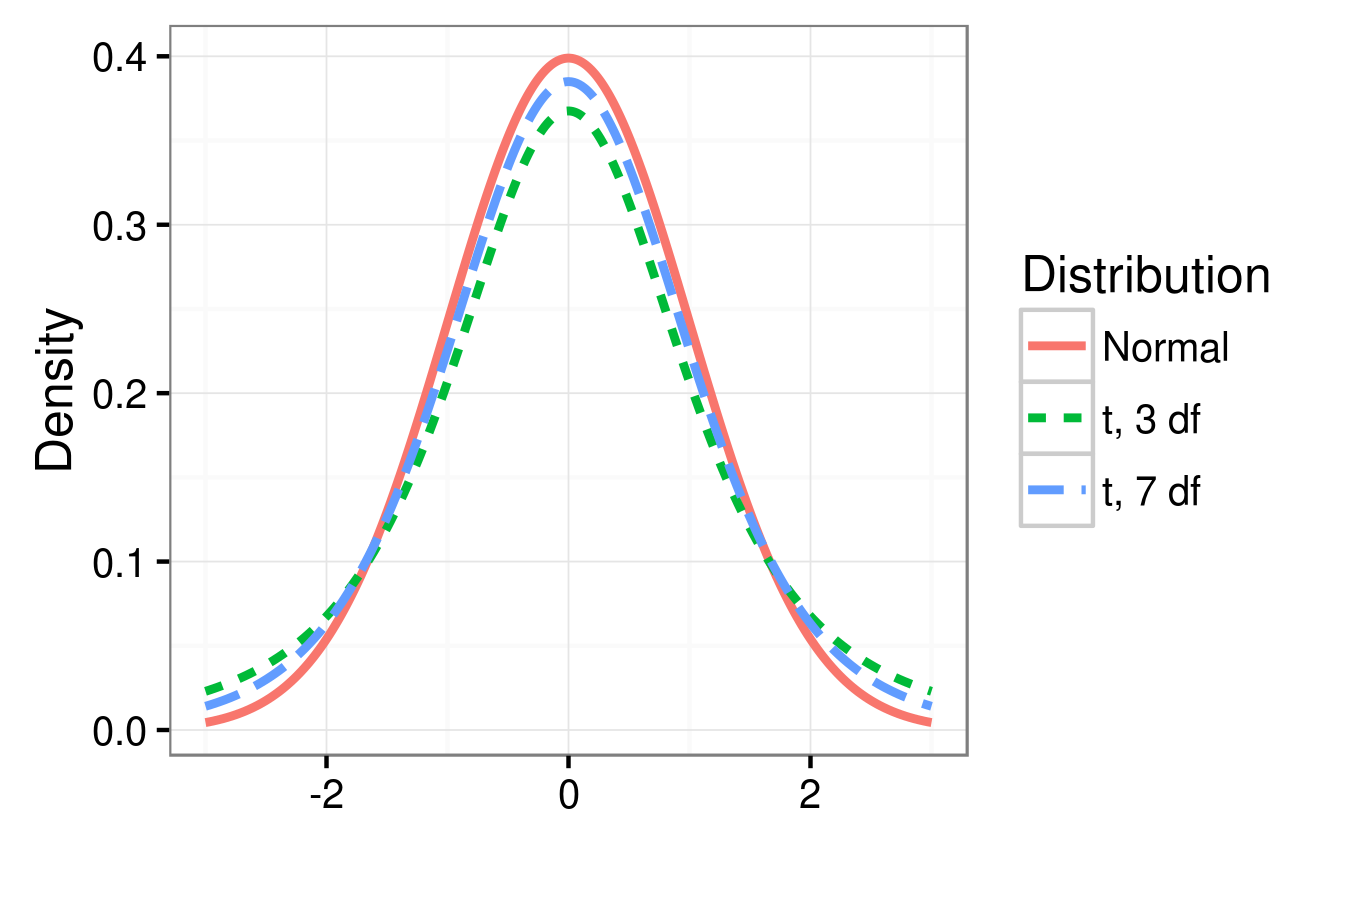
\includegraphics[width=4.5in]{../images/ch7_t_dist}
\par}
\end{frame}

\begin{frame}{t distribution critical values}
\begin{block}{}
\large
Critical values from t distributions can be found in tables (Table A-3) or in the StatCrunch ``T" calculator.\\
\pause\medskip
Then, confidence interval can be calculated by,
\[CI = \bar x \pm t_{\alpha/2, df} \Paren{\frac s {\sqrt n}}\]
where $t_{\alpha/2, df}$ is the critical $t$ value at $\alpha/2$ and $df=n-1$ and $s$ is the sample standard deviation.
\end{block}
\end{frame}

\begin{frame}{Confidence intervals for means, summary}
\begin{block}{}
\large
If population is normally distributed, or sample size is 30 or greater,
\begin{itemize}
\pause\item If population standard deviation $\sigma$ is known, confidence intervals are constructed with $z$ distribution critical values and $\sigma$ for standard deviation.
\pause\item If population standard deviation is \bt{not} known, confidence intervals are constructed with $t$ distribution critical values and sample standard deviation $s$ for standard deviation.
\end{itemize}
\pause Otherwise, if population is not normally distributed and sample size is less than 30, valid confidence intervals can not be constructed using these methods.
\end{block}
\end{frame}

\begin{frame}{Confidence intervals of means in StatCrunch}
\begin{block}{}
\large
\begin{itemize}
\item Stat $\to$ Z Stats \bt{or} T Stats $\to$ One Sample $\to$ With Summary \bt{or}\\T Stats $\to$ One Sample $\to$ With Data
\item For known population standard deviation (Z Stats): Enter ``Sample mean", ``Standard deviation" and ``Sample Size" 
\item For unknown population standard deviation (T Stats): Enter ``Sample mean", ``Sample std. dev." and ``Sample Size" (not degrees of freedom)
\item For data set (T Stat with Data): Select column which contains data
\item Select ``Confidence interval for $\mu$"
\item Enter confidence level if different than 0.95.
\item Click ``Compute!"
\item The confidence interval is found in ``L. Limit" and ``U. Limit"
\end{itemize}
\end{block}
\end{frame}


\begin{frame}{Confidence intervals for means, example}
\begin{exampleblock}{Example}
TACO would like to know, among people who eat tacos, how many tacos per week they eat. They survey 36 taco eaters and get a sample mean of 5.4 tacos per week with a standard deviation of 2.7. What is a 90\% confidence interval for the population mean number of tacos eaten?
\begin{itemize}
\pause\item A 90\% level of confidence means that $\alpha = 0.10$.
\pause\item It is unknown if number of tacos eaten is normally distributed (probably not), but our sample size is above 30, so we can treat the sampling distribution as normal.
\pause\item Since population standard deviation is unknown, we will use $t$ distribution critical values with degrees of freedom of $n-1=35$, $t_{\alpha/2, df}= t_{0.05,35} = 1.69$.
\pause\item $\ds CI = \bar x \pm t_{\alpha/2}\Paren{\frac s {\sqrt{n}}} = 5.4 \pm (1.69) \Paren{\frac {2.7}{\sqrt{36}}} = 5.4 \pm 0.76$\\
\pause\smallskip
{\large $\bv{(4.64, 6.16)}$ \par}
\end{itemize}
\end{exampleblock}
\end{frame}

\begin{frame}{Confidence intervals for means, example}
\begin{exampleblock}{Example}
Recall, in the United States adult men have a mean height of 69.2 inches with a standard deviation of 5.79 inches.\\
\medskip
The heights from a sample of 40 male Metro State students are measured. The mean height from the sample is 66.3 inches. What is a 95\% confidence interval for the mean height of Metro State students?
\begin{itemize}
\pause\item A 95\% level of confidence means that $\alpha = 0.05$.
\pause\item We can assume that the heights of Metro State students have the same standard deviation as the general US population, $\sigma = 5.79$.
\pause\item Since we know the population standard deviation, we will use $z$ distribution critical values, $z_{\alpha/2} = 1.96$.
\pause\item $\ds CI = \bar x \pm z_{\alpha/2}\Paren{\frac \sigma {\sqrt{n}}} = 66.3 \pm (1.96) \Paren{\frac {5.79}{\sqrt{40}}} = 66.3 \pm 1.794$\\
\pause\smallskip
{\large $\bv{(64.506, 68.094)}$ \par}
\end{itemize}
\end{exampleblock}
\end{frame}

\begin{frame}{Confidence intervals for means, example}
\begin{exampleblock}{Example}
With a confidence interval of $(64.51, 68.01)$, can we conclude that the heights of Metro State students are different than the general US population?
\begin{itemize}
\pause\item Since the US mean height of 69.2 inches is not in our interval, we can conclude (with 95\% certainty) that the heights of Metro State students differ from the general population.
\end{itemize}
\end{exampleblock}
\end{frame}


\begin{frame}{Find needed sample size}
\begin{block}{}
\large
To calculated the sample size needed for a desired margin of error,
\[n = \frac{z_{\alpha/2} \times \sigma}{ME}\]
\begin{itemize}
\pause\item Because sample size calculations are done before data is gathered, so value for standard deviation must be known or estimated.
\pause\item Because $t$ distribution values depend of sample size, they are difficult to work with while calculating sample size. Thus, $z$ critical values are generally used.
\end{itemize}
\end{block}
\end{frame}

\begin{frame}{Find needed sample size with StatCrunch}
\begin{block}{}
\begin{itemize}
\item Stat $\to$ Z Stats $\to$ One Sample $\to$ Width/Sample Size
\item Enter ``Confidence level" if different than 0.95.
\item Enter estimated or given standard deviation as ``Std. dev."
\item Enter twice desired margin of error as ``Width" 
\item Click ``Compute!"
\item The needed sample size is found in ``Sample size"
\end{itemize}
\end{block}

\end{frame}

\begin{frame}{Find needed sample size, example}
\begin{exampleblock}{Example}
\large
Recall, in the United States, adult women have a mean height of 63.7 in with a standard deviation of 5.96 in. If we wanted to find the mean height of female students at Metro State within plus or minus 1.5 inches at a 99\% confidence level, how many students would need to be included in the sample?

\begin{itemize}
\pause\item A 99\% level of confidence means that $\alpha = 0.01$.
\pause\item $\ds n = \Paren{\frac{z_{\alpha/2} \times \sigma}{ME}}^2= \Paren{\frac{2.576 \times 5.96}{1.5}}^2 = 104.76 \to 105$
\end{itemize}
\end{exampleblock}
\end{frame}

\begin{frame}<handout:0>{Group work}
\begin{block}{}
\large
\begin{itemize}
\item Complete question 2, all parts.
\end{itemize}
\end{block}
\end{frame}


\end{document}